% !TEX encoding = UTF-8 Unicode
% !TEX root =  ../Bachelorarbeit.tex

%++++++++++++++++++++++++++++++++++++++++++++++++++++++++++++++++++++++++++++++++++++++++++++++++++++%

\chapter{Fazit und kritische Bewertung}
\label{cha:Fazit}

Im Rahmen dieser Arbeit wurde eine interruptgesteuerte Benutzerschnittstelle f\"ur den Mikrocontroller MSP430FR5729 konzipiert und implementiert. Zentrale Komponente ist das sogenannte Observer-Modul, welches sowohl den Empfang als auch die statusbasierte Verarbeitung externer Steuerbefehle \"ubernimmt. Damit bildet es eine funktionale Schnittstelle zwischen dem Mikrocontroller, seinem Hauptprogramm und der Benutzerinteraktion.

%====================================================================================================%

\section{Das Ergebnis}
\label{sec:Ergebnis}

Die Entwicklung wesentlicher Bausteine, insbesondere die der Timer-Interrupt-Service-Routine (Timer-ISR), UART-Kommunikationsschnittstelle (UART-ISR) sowie der statusorientierten Abarbeitung eingehender Befehle, legt eine flexible und erweiterbare Basis f\"ur zuk\"unftige Funktionsimplementierungen. Die exemplarisch realisierten Lese- und Schreibfunktionen demonstrieren die praktische Anwendbarkeit dieser Architektur.

Ein bedeutendes Ergebnis stellt die Realisierung des Observer-Moduls f\"ur Debugging-Zwecke dar, welches unabh\"angig von der \"ublichen Entwicklungsumgebung (Code Composer Studio und MSP-FET) agiert. Dies erlaubt es dem Benutzer, unter Realbetriebsbedingungen, tiefgreifende Analysen durch das auslesen und beschreiben von Speicherzellen w\"ahrend der aktiven Laufzeit. Gerade bei der Entwicklung auf Mikroprozessoren -- wie dem MSP430 -- sind Stichproben unter Echtzeitbedingungen von hohem Wert, da kontrolliert und nicht blockierend auf Speicherzellen zugegriffen werden kann.

Im Anschluss an die Implementierung wurde besonderes Augenmerk auf die Analyse der Systemreaktivit\"at gelegt. Zu diesem Zweck wurden Laufzeitmessungen durchgef\"uhrt, welche aufzeigen, inwieweit die entwickelten Komponenten den Anforderungen an Echtzeitf\"ahigkeit gen\"ugen. Das folgende Kapitel beschreibt detailliert die zugrunde liegende Methodik und pr\"asentiert die ermittelten Messergebnisse.\AI


%----------------------------------------------------------------------------------------------------%

\subsection{Untersuchung der Laufzeit unter Realbedingungen}
\label{laufzeit}

Zur Untermauerung der in Kapitel~\ref{konzept_status_&_interrupt} genannten Vorteile eines statusorientierten Zustandsautomaten hinsichtlich der Systemreaktivit\"at sind Laufzeituntersuchungen unerl\"asslich. Diese Messungen erm\"oglichen eine fundierte Bewertung der Ausf\"uhrungszeiten hinsichtlich genannter Vor- und Nachteile f\"ur andere Softwarekomponenten und Systemzust\"ande.

Die Erfassung und Auswertung der Laufzeiten erfolgte mittels eines Digital-Oszilloskops (Modell: PicoScope 3406D MSO) in Verbindung mit der zugeh\"origen Messsoftware PicoScope 7 T\&M. F\"ur die Aufzeichnung der Signale wurde der digitale Eingang \Code{D1} des Oszilloskops genutzt. Eine einheitliche Abtastrate von 500 \Abkuerzung{Mega-Samples pro Sekunde}{MS/s} (Mega-Samples pro Sekunde) wurde f\"ur alle Messungen verwendet, um eine hohe zeitliche Aufl\"osung sicherzustellen.

Zur Signalisierung der Messintervalle wurden GPIO-Pins von Port 3 des zugrundeliegenden Mikrocontrollers verwendet. Die exakte Zeitmessung einzelner Codeabschnitte erfolgte durch das Setzen eines spezifischen GPIO-Pins (konkret \Code{P3.4}, adressiert \"uber \Code{BIT4} des \Code{P3OUT}-Registers) zu Beginn des zu messenden Abschnitts (\Code{SETBIT(P3OUT, BIT4);}) und dessen unmittelbares Zur\"ucksetzen (\Code{CLRBIT(P3OUT, BIT4);}) an dessen Ende (\Vgl \Abbildung{read_mem_function} und \Abbildung{write_mem_function}). Dieses Verfahren erm\"oglicht eine pr\"azise Erfassung der Ausf\"uhrungsdauer sowohl einzelner Verarbeitungszyklen als auch kompletter Lese- oder Schreiboperationen.

Die nachfolgende \Tabelle{laufzeitmessungen} fasst die ermittelten Laufzeiten f\"ur repr\"asentative Ereignisse und Funktionen innerhalb des Observer-Moduls zusammen.

\begin{table}[h!]
	\small
	\centering
	\begin{tabular}{|l|l|l|}
		\hline
		\textbf{Ereignis} & \textbf{Funktion} & \textbf{Laufzeit} \\\hline
		Leerlauf & TIMER0\_B0\_ISR & $\sim$3{,}9~\textmu s \\
		Time-Out Timer & state\_0 & $\sim$3{,}4~\textmu s \\
		Befehlsinterpretation & state\_1 & $\sim$70 - 140~ms \\
		Resetzustand & state\_2 & $\sim$6{,}3~\textmu s \\
		Leseoperation f\"ur 13 Byte & read\_mem & $\sim$130~ms \\
		Leseoperation Parameterentnahme & read\_mem & $\sim$240~\textmu s \\
		Leseoperation pro Byte & read\_mem & $\sim$10~\textmu s (+ $\sim$10~ms ISR Zyklus) \\
		Schreiboperation f\"ur "test" & write\_mem & $\sim$40~ms \\
		Schreiboperation Parameterentnahme & write\_mem & $\sim$220~\textmu s \\
		Schreiboperation pro Byte & write\_mem & $\sim$10~\textmu s (+ $\sim$10~ms ISR Zyklus) \\\hline
	\end{tabular}
	\caption{Laufzeitmessungen -- Observer-Modul State-Machine}
	\label{tab:laufzeitmessungen}
\end{table}

Ein wesentliches Ergebnis der statusorientierten, zeichenweisen Verarbeitung ist die Freigabe von Rechenzeit zwischen den einzelnen Verarbeitungszyklen f\"ur andere Systemaufgaben. \Abbildung{zeichenorientiertes_lesen} visualisiert diesen Sachverhalt exemplarisch anhand einer Leseoperation. Jeder in der Abbildung dargestellte Impuls repr\"asentiert die Verarbeitungszeit f\"ur ein einzelnes Zeichen. Die dargestellte Operation (\Code{rdm 0x1C00 13}) weist insgesamt 14 solcher Impulse auf. Der initiale Impuls zeigt die l\"angste Dauer, welche aus der einmaligen Initialisierungsphase pro Leseoperation resultiert: Hierbei werden die erforderlichen Parameter (Speicheradresse, Anzahl der Bytes) aus dem \Code{uart\_buffer} extrahiert. Dieser Vorgang involviert rechenzeitintensive String-Operationen wie \Code{strtok}, \Code{strlen}, \Code{strtol} und \Code{atoi}. Die nachfolgenden Zyklen, welche die eigentliche zeichenweise Leseoperation des Zeichens umfassen, weisen signifikant k\"urzere Ausf\"uhrungszeiten von etwa 10~\textmu s auf. In den Intervallen -- von ca. 10~ms -- zwischen diesen aktiven Verarbeitungsphasen (bedingt durch die Periode der Timer-ISR) steht der Prozessor f\"ur andere Aufgaben -- wie beispielsweise der Ausgabe des gelesenen Zeichens -- zur Verf\"ugung. Der letzte Verarbeitungszyklus (im Beispiel der 14.) dient der Finalisierung der Leseoperation. Er beinhaltet die erfolgreiche Pr\"ufung auf die angeforderte Anzahl an gelesenen Zeichen (Abgleich von \Code{mem\_addr\_idx} mit \Code{blocks} in der \Code{read\_mem}-Funktion \Vgl \Abbildung{read_mem_function}), und leitet bei Erfolg den \"Ubergang in den R\"ucksetzzustand (\Code{state\_2}) durch Aktualisierung des \Code{state\_ptr} ein.\AI

\begin{figure}[h!]
	\centering
	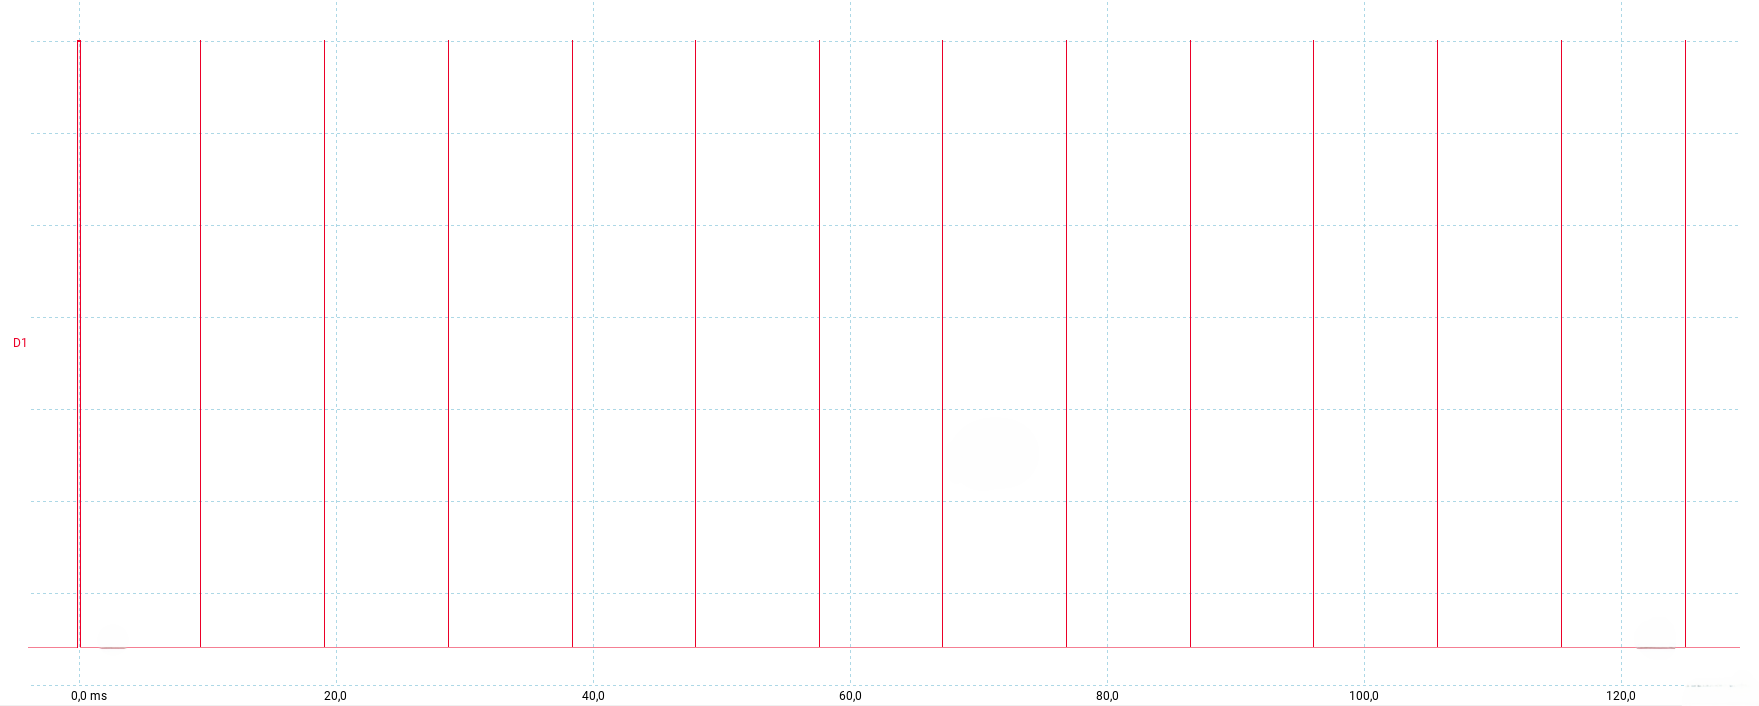
\includegraphics[width=0.8\textwidth]{../Bilder/BA_MSP430_Observer_Zeitmessungen/ReadMem_Complete_zoomed_rdm_0x1C00_13.png}
	\caption{Oszillogramm einer vollst\"andigen Speicherleseoperation (\Code{rdm 0x1C00 13})}
	\label{fig:zeichenorientiertes_lesen}
\end{figure}

Auch die in Kapitel~\ref{Entwicklung} beschriebenen Vorteile der Integration softwarebasierter Breakpoints -- insbesondere f\"ur kritische Operationen wie das Lesen und Schreiben auf Speicherzellen -- konnten im Verlauf der Entwicklung best\"atigt werden. Die in Kapitel~\ref{Hardware_VS_Software_Breakpoints} begonnene Konzeptausarbeitung liefert eine fundierte Grundlage f\"ur die folgende Bewertung dieser Mechanismen.

%----------------------------------------------------------------------------------------------------%

\subsection{Fazit zu Software Breakpoints}
\label{sec:FazitSoftwareBreakpoints}

Die Realisierung von Software-Breakpoints auf dem Low‑Power‑Mikrocontroller MSP430FR5729 erfordert ein tiefgehendes Verst\"andnis der Prozessor‑Architektur, der Instruktionsformate, der vielf\"altigen Adressierungs-Modi und ihrer Auswirkungen auf die Speicherverwaltung und der nebenl\"aufigen Abl\"aufe im System. Die Analyse der Problemstellung hat ergeben, dass unter anderem kritische Bereiche atomar bearbeitet, Register und Stack-Zust\"ande zuverl\"assig gesichert und Intrinsics korrekt eingesetzt werden m\"ussen. Zudem sind umfangreiche Funktionen zur \"uberwachung und Protokollierung des Systemzustands zu implementieren.

Die erwartete komplexit\"at inklusive der Anforderungen an Robustheit, Echtzeitf\"ahigkeit und m\"oglichst geringem Eingriff in den Betrieb \"uberschreitet den Rahmen einer \"ublichen Bachelorarbeit. Eine vollst\"andige, ausgereifte Implementierung w\"are mit dem Umfang einer Masterarbeit oder vergleichbarer Forschungsarbeiten m\"oglich. Dennoch bildet dieses Thema eine exzellente Grundlage f\"ur weiterf\"uhrende Arbeiten in den Bereichen eingebettete Echtzeitsysteme und Debugging‑Technologien, insbesondere in Bezug auf Architekturen mit flexiblen, aber komplexen Speicheradressierungsmechanismen.

%====================================================================================================%

\newpage
\section{Die Bewertung}
\label{sec:Bewertung}
Die zeitkritische Synchronisation zwischen Hauptprogramm und Observer-Modul stellte eine zentrale Herausforderung dar -- insbesondere im Hinblick auf den gew\"ahlten, nicht-blockierenden Ansatz der statusorientierten Verarbeitung. Die sequentielle, zeichenweise Abarbeitung von Lese- und Schreiboperationen \"uber mehrere Verarbeitungsschritte hinweg erh\"ohte zwar die Komplexit\"at der Implementierung, f\"uhrte jedoch zu einer \"au{\ss}erst performanten L\"osung hinsichtlich der Systemreaktivit\"at. Dies ist insbesondere f\"ur ein als \grqq unsichtbares\grqq Plug-in-Modul konzipiertes System essenziell.

Die vollst\"andige Implementierung softwaregesteuerter Breakpoints erwies sich hingegen als sehr anspruchsvoll. Zwar konnte ein vielversprechender Ansatz gem\"a{\ss} dem in Kapitel~\ref{ImplementierungSoftwareBreakpoints} skizzierten Konzept entwickelt werden, (\Vgl Abbildung~\ref{fig:software_breakpoint}) jedoch gelang keine vollst\"andig funktionale, robuste und konsistente Einbindung zur Laufzeit. Der entsprechende Quellcode befindet sich weiterhin, wenn auch auskommentiert, im Observer-Modul.

\begin{figure}[h!]
	\centering
	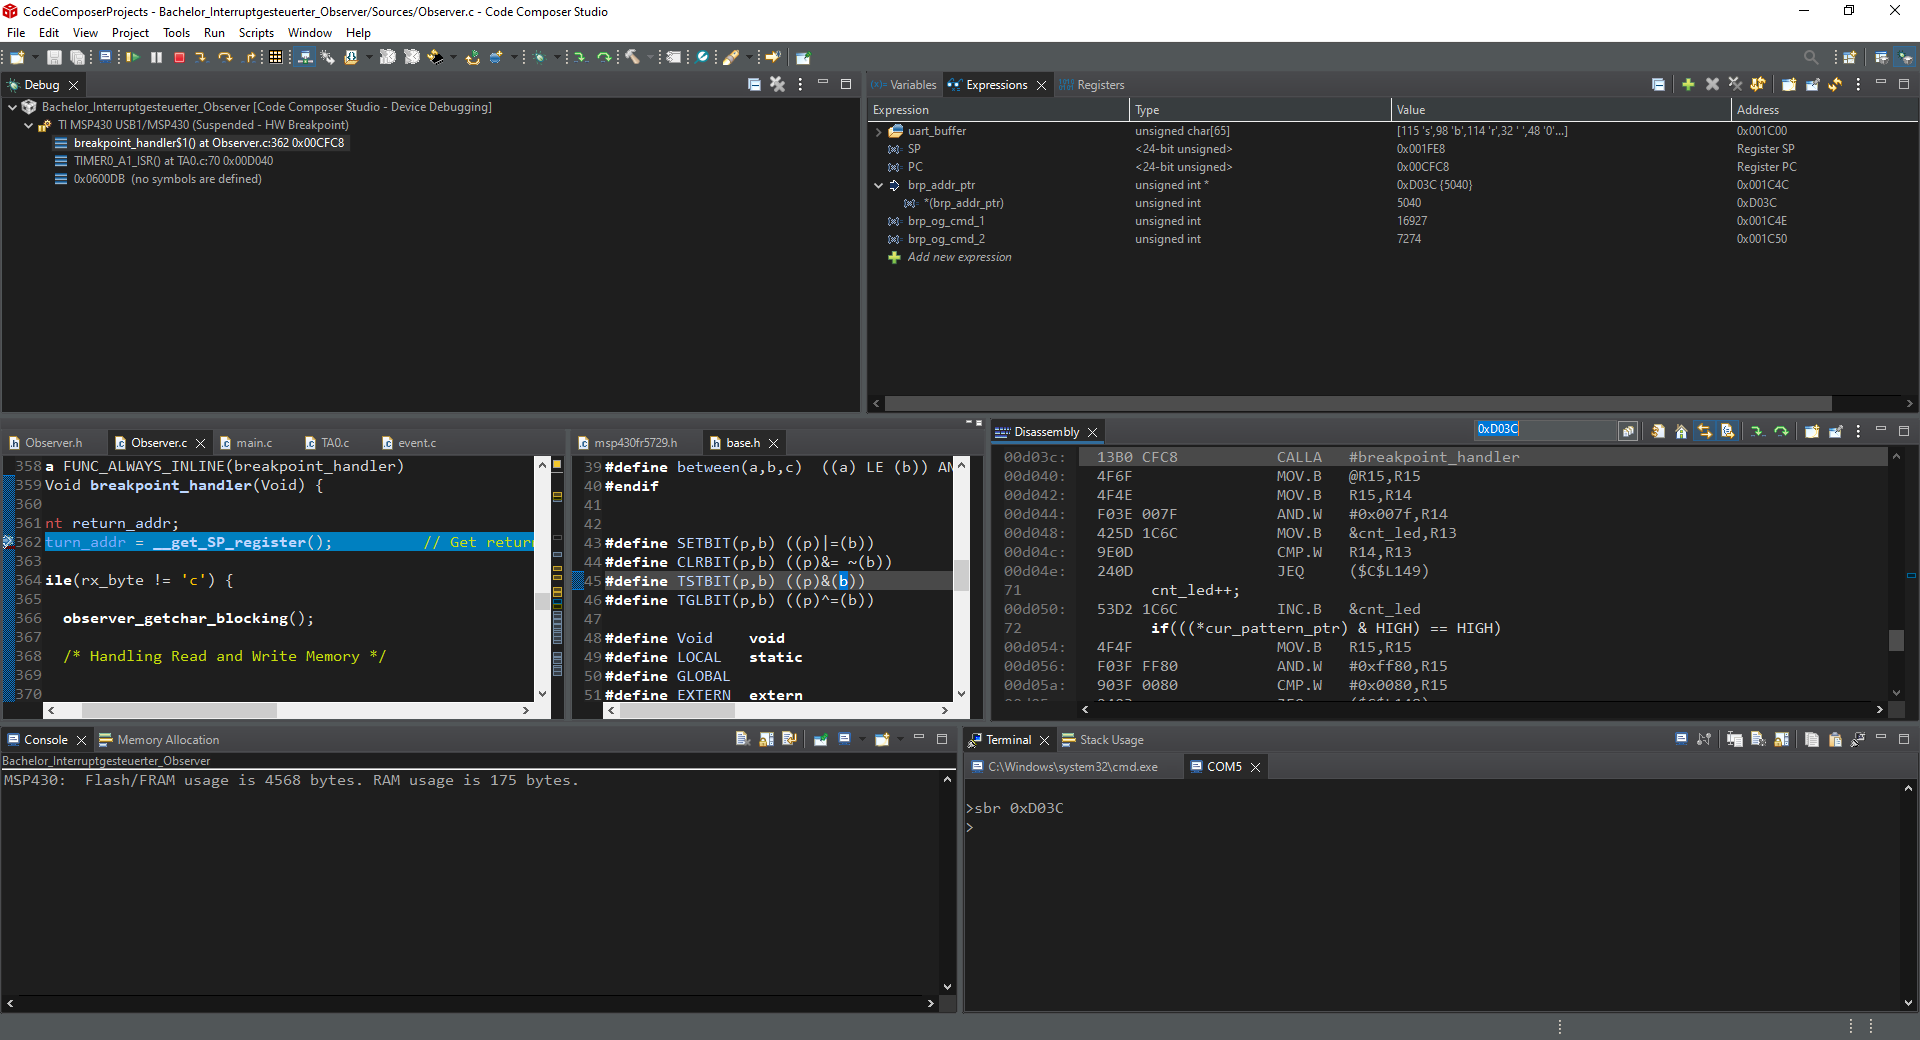
\includegraphics[width=0.7\textwidth]{../Bilder/ObserverModule/set_breakpoint.png}
	\caption{Setzen eines Software-Breakpoints an einer frei ausgew\"ahlten Speicheradresse im Stack -- \Code{sbr 0xD03C}}
	\label{fig:software_breakpoint}
\end{figure}

Nichtsdestotrotz konnte durch die umfassend durchgef\"uhrte Laufzeitanalyse die Echtzeitf\"ahigkeit des Observer-Moduls best\"atigt werden. Diese wird allerdings mit einem erh\"ohten Speicherverbrauch erkauft, bedingt durch den Einsatz nicht vollst\"andig optimierten Codes und speicherintensiver Funktionen der Standard-String-Bibliothek.

Ein wesentliches Manko stellt die aktuelle Beeintr\"achtigung der UART-Schnittstelle dar. Aufgrund der nicht implementierten automatischen Baudratenerkennung -- wie in Kapitel~\ref{auto_baud} kurz beleuchtet wurde -- kann das Hauptprogramm diese Schnittstelle nicht parallel nutzen. Dies steht dem Anspruch entgegen, das Observer-Modul vollst\"andig vom restlichen System zu entkoppeln, da ansonsten ein zentrales Modul f\"ur Kommunikationsmanagement zur Konfliktvermeidung erforderlich w\"are.\AI

%====================================================================================================%

\section{Ein Ausblick}
\label{sec:EinAusblick}

Der modulare Aufbau des Systems, kombiniert mit der flexiblen Konfiguration der Timer- und UART-Interrupts, bietet eine solide Grundlage f\"ur die Integration weiterf\"uhrender Funktionalit\"aten. Insbesondere die strukturierte Umsetzung und umfangreiche Analyse der Software-Breakpoint-Mechanismen liefert wertvolle Impulse f\"ur zuk\"unftige Arbeiten im Bereich experimenteller Debugging-Techniken.

Ein weiterer Entwicklungsschritt k\"onnte die Implementierung eines weiteren Moduls zur automatischen Baudratenerkennung darstellen. Diese w\"urde es erm\"oglichen, die UART-Schnittstelle sowohl f\"ur interne als auch externe Kommunikationsprozesse effizient zu nutzen, ohne die Systemtrennung aufzugeben.

Langfristig k\"onnte die entwickelte Architektur auch in komplexere, multitaskingf\"ahige Systeme \"uberf\"uhrt werden. Durch den nicht-blockierenden und zustandsbasierten Aufbau ist das Observer-Modul pr\"adestiniert f\"ur eine Integration in reaktive, ereignisgesteuerte Steuerungsplattformen zur Erg\"anzung bereits vorhandener Debugging-Mechanismen.